%%%%%%%%%%%%%%%%%%%%%%%%%%%%%%%%%%%%%%%%%%%%%%%%%%%%%%%%%%%%%%%%%%
%%%%%%%%%%    Do not touch the below 70 lines     %%%%%%%%%%%%%%%%
%%%%%%%%%%%%%%%%%%%%%%%%%%%%%%%%%%%%%%%%%%%%%%%%%%%%%%%%%%%%%%%%%%
\documentclass[11pt,a4paper,onecolumn,oneside]{report}

\usepackage{mathptmx}
\usepackage[T1]{fontenc}
\usepackage[utf8]{inputenc}

\RequirePackage[top=3cm, bottom=1in, left=1in, right=1in]{geometry}
\linespread{1.3}

\usepackage{titlesec}
\usepackage{amsmath}
\usepackage{amssymb}
\usepackage{mathtools}
\usepackage{enumerate}
\usepackage{bbm}
\usepackage{algorithm}
\usepackage{algorithmic}
\usepackage{epsfig}
\usepackage{color}
\usepackage{graphicx}
\usepackage{caption}
\usepackage{subcaption}
\usepackage{cases}
\usepackage{url}
\usepackage{cite}
\usepackage{fancyhdr}
\usepackage{tocloft}
\usepackage{pdfpages}
\usepackage{adjustbox}
\usepackage{indentfirst}
\usepackage{tocloft}

\newlength{\mylen}

\renewcommand{\cftfigpresnum}{\figurename\enspace}
\renewcommand{\cfttabpresnum}{\tablename\enspace}
\renewcommand{\cftfigaftersnum}{:}
\renewcommand{\cfttabaftersnum}{:}
\settowidth{\mylen}{\cftfigpresnum\cftfigaftersnum}
\settowidth{\mylen}{\cfttabpresnum\cfttabaftersnum}
\addtolength{\cftfignumwidth}{\mylen}
\addtolength{\cfttabnumwidth}{\mylen}

\setcounter{secnumdepth}{3}
\setcounter{tocdepth}{3}

\renewcommand\cftsecafterpnum{\vskip15pt}
\renewcommand\cftsubsecafterpnum{\vskip15pt}
\renewcommand\cftfigafterpnum{\vskip15pt}
\renewcommand{\thesection}{\Roman{section}.}
\renewcommand{\thesubsection}{\arabic{section}.\arabic{subsection}.}
\renewcommand{\thesubsubsection}{\arabic{section}.\arabic{subsection}.\arabic{subsubsection}.}
\renewcommand{\contentsname}{\hfill\bfseries\Large Contents\hfill}   
\renewcommand{\listfigurename}{\hfill\bfseries\Large List of Figures\hfill}
\renewcommand{\listtablename}{\hfill\bfseries\Large List of Tables\hfill}
\renewcommand{\thefigure}{\arabic{figure}}
\newcommand{\qed}{\hfill\blacksquare}
\renewcommand{\bibname}{\hfill\bfseries\Large References \hfill\hfill}
\renewcommand{\abstractname}{\bfseries\Large Abstract \hfill\hfill}

\captionsetup{figurename=Figure,labelsep=period}
\captionsetup{tablename=Table,labelsep=period}

%%%\hyphenpenalty=9000

\newcounter{lemma}
\newcounter{proposition}
\newcounter{theorem}
\newtheorem{lemma}{\bf Lemma}
\newtheorem{proposition}{\bf Proposition}
\newtheorem{theorem}{\bf Theorem}
\newtheorem{proof}{\bf Proof}

%\input{mymath_mod.tex}


\newcommand{\HIGH}[1]{{\textcolor{blue}{#1}}}
%\renewcommand{\baselinestretch}{1.5} 

\DeclareMathOperator*{\argmax}{arg\,max}

\fancyhf{}
\renewcommand{\headrulewidth}{0pt}
\cfoot{\thepage}
\pagestyle{fancy}
%\pagenumbering{gobble}

\begin{document}

%%%%%%%%%%%%%%%%%%%%%%%%%%%%%%%%%%%%%%%%%%%%%%%%%%%%%%%%%%%%%%%%%%
%%%%%%%%%%    Do not touch the above 70 lines     %%%%%%%%%%%%%%%%
%%%%%%%%%%%%%%%%%%%%%%%%%%%%%%%%%%%%%%%%%%%%%%%%%%%%%%%%%%%%%%%%%%


%%%%%%%%%%%%%%%%%%%%%%%%
%%%%%% Front cover
%%%%%%%%%%%%%%%%%%%%%%%%
\begin{center}
\LARGE Doctoral Thesis
% or Ph.D...

\vspace{3cm}
\huge Enhanced Fidelity of Monte Carlo Coupled Multi-Physics Simulations for Light Water Reactors

\vfill

\LARGE Muhammad Imron

\vspace{2cm}

\LARGE Department of Nuclear Engineering 
% Department of Computer Science and Engineering

\vspace{2cm}

\LARGE Ulsan National Institute of Science and Technology
\vspace{2cm}

\LARGE 2024

\end{center}
\thispagestyle{empty}
\clearpage

%%%%%%%%%%%%%%%%%%%%%%%%
%%%%%% TITLE PAGE
%%%%%%%%%%%%%%%%%%%%%%%%
\begin{center}
\hbox{ }

\hbox{ }

\huge Enhanced Fidelity of Monte Carlo Coupled Multi-Physics Simulations for Light Water Reactors 

\vspace{5cm}

\LARGE Muhammad Imron

\vspace{6cm}

\LARGE Department of Nuclear Engineering 

\vspace{2cm}

\LARGE Ulsan National Institute of Science and Technology

\end{center}
\thispagestyle{empty}
\clearpage

%%%%%%%%%%%%%%%%%%%%%%%%%%%%%%%%%%%%%%%%%%%%%
%			THESIS APPROVAL
%%%%%%%%%%%%%%%%%%%%%%%%%%%%%%%%%%%%%%%%%%%%%

% [Thesis approval]
% Add the approval doc signed by your advisor in a PDF file
% Put your pdf with the filename below, and uncomment it.
%\includepdf[fitpaper= true, pages=-]{sample_approval.pdf}

% [Confirmation of thesis approval]
% add the certificate signed by your committee in a PDF file
% Put your pdf with the filename below, and uncomment it.
%\includepdf[fitpaper= true, pages=-]{sample_confirmation.pdf}

%%%%%%%%%%%%%%%%%%%%%%%%%%%%%%%%%%%%%%%%%%%%%
%			ABSTRACT
%%%%%%%%%%%%%%%%%%%%%%%%%%%%%%%%%%%%%%%%%%%%%
\begin{abstract}
% \begin{center}
% \large Enhanced Fidelity of Monte Carlo Coupled Multi-Physics Simulations for Light Water Reactors 
% \end{center}
\vspace{1cm}

This study presents a framework to enhance the fidelity of typical Monte Carlo (MC) coupled multi-physics simulations for Light Water Reactors (LWRs) through two key improvements. First, the introduction of multi-physics simulations with spatially continuous material properties using the Functional Expansion Tally (FET) combined with delta-tracking. Second, the incorporation of on-the-fly thermal expansion of reactor core components during MC particle tracking. In direct multi-physics coupled MC simulations, the use of spatially continuous material properties is  particularly crucial to accurately modeling spatial self-shielding effects, which depend on smooth intra-fuel-pellet temperature distributions. The significant reduction in discretization also preserves the MC method's advantage in handling continuous geometry. Additionally, modeling thermal expansion is essential because the geometric data of reactor components is typically provided at room temperature, while reactors operate at much higher temperatures. Numerical experiments are conducted to assess the applicability and advantages of the proposed multi-physics framework across a range of reactor core problems, from two-dimensional pin-cell to whole-core reactor problems.

The incorporation of spatially continuous material properties produces solutions that asymptotically converge to those from conventional cell-based discretized simulations with infinitesimally small cells as demonstrated in the two-dimensional pin-cell problem. Similar outcomes are observed in three-dimensional pin cell and assembly problems, where the continuous representation of material properties results in more accurate solutions for both eigenvalue and axial power distributions, compared to the conventional cell-based discretization method. In typical whole-core LWR problems, the proposed method reproduces high-fidelity solutions for both eigenvalue and pin powers, while reducing simulation times by around threefold and requiring 80\% less memory than the traditional cell-based discretization using very small cells.

Whereas the numerical results for on-the-fly thermal expansion demonstrates that the observed trends in reactivity differences due to thermal expansion for varying boron concentrations and fuel temperatures align with previous studies. Additionally, the calculated Isothermal Temperature Coefficients (ITC) show improvement when thermal expansion is considered. Using core-averaged temperatures for expansion provides fairly accurate results, but employing local temperatures at pin levels can enhance accuracy further. Moreover, incorporating thermal expansion also improves solutions for depletion problems, especially at high power and high fuel burnup. These findings suggest that integrating the proposed framework into reactor modeling can significantly enhance simulation fidelity. Therefore, the framework has the potential to be incorporated into future Monte Carlo production codes to meet the growing demands for improved reactor safety.

\vfill
\end{abstract}

\clearpage

%%%%%%%%%%%%%%%%%%%%%%%%%%%%%%%%%%%%%%%%%%%%%%%%%%%%%%%%%%%%% 
%%%%%%%%%%    Do not touch the below 20 lines 
%%%%%%%%%%%%%%%%%%%%%%%%%%%%%%%%%%%%%%%%%%%%%%%%%%%%%%%%%%%%% 
%%% The following page is intentionally left as blank
%%% White attachment form
\hbox{ }
\thispagestyle{empty}
\clearpage

%%% Table of Contents
\tableofcontents{}
\thispagestyle{empty}
\vfill
\clearpage

%%% List of Figures
\listoffigures
\thispagestyle{empty}
\clearpage

%%% List of Tables
\listoftables
\thispagestyle{empty}
\clearpage

%%% reset page numbering
\setcounter{page}{1}
%%%%%%%%%%%%%%%%%%%%%%%%%%%%%%%%%%%%%%%%%%%%%%%%%%%%%%%%%%%%% 
%%%%%%%%%%    Do not touch the above 20 lines 
%%%%%%%%%%%%%%%%%%%%%%%%%%%%%%%%%%%%%%%%%%%%%%%%%%%%%%%%%%%%% 



%%%%%%%%%%%%%%%%%%%%%%%%%%%%%%%%%%%%%%%%%%%%%
%			Introduction
%%%%%%%%%%%%%%%%%%%%%%%%%%%%%%%%%%%%%%%%%%%%%
\section{Introduction} \label{s1}

Over the past five decades, advancements in modern computing have enabled direct whole-core Monte Carlo (MC) coupled multi-physics simulations for large-scale Light Water Reactors (LWRs). In this approach, the multi-physics coupling between MC codes and thermal-hydraulic (TH) solvers is accomplished at the pin-by-pin level. Numerous examples of these reactor multi-physics simulations can be found in the literature \cite{tung_2020,kelly_2017,ma_2019}, and they had demonstrated that such simulations are practically feasible for academic and research purposes. The results from such reactor multi-physics simulations have shown improved accuracy when compared to measured data and are often used as reference solutions for lower-order deterministic codes. However, according to Smith and Forget \cite{smith_2013}, there are still many important aspects of LWR simulations that must be incorporated to produce truly high-fidelity analysis tools.

While the work of Smith and Forget highlights many aspects to improve the fidelity of reactor calculations, this thesis attempts to solve two issues. They are: first, inadequate spatial resolution, such as the improper modeling of radial temperature variations in fuel pellets, which is essential for accurately modeling spatial self-shielding effects \cite{smith_2013, nchoi_2020}. Second, thermal expansion of the reactor core materials, which is often neglected in typical direct whole-core MC coupled multi-physics simulations. The subsequent subsections, \ref{sec11} and \ref{sec12}, will discuss each of these aspects in detail. Additionally, a literature review for each aspect is described in those subsections.

\subsection{Spatial Resolution} \label{sec11}

One of the main advantages of the MC methodology is its ability to handle continuous geometry within a single material. However, when conducting MC multi-physics reactor simulations, it is necessary to discretize the problem domain into smaller cells, even within the same material. The material properties, such as fuel temperature, moderator density, and the isotopic composition of materials diluted in the moderator, are assumed to be uniform within each cell. This discretization is essential for achieving adequate spatial resolution and accurately modeling variations in material properties.

Figure \ref{fig_1} shows the axial view of a typical MC geometry model for a single fuel pin. The actual geometry consists of the fuel, gap, cladding, and coolant, as illustrated in Figure \ref{fig_1a}. For multi-physics simulations, this geometry must be discretized into several cells both radially and axially, as shown in Figure \ref{fig_1b}, even though the actual geometry is relatively simple.

Although high spatial resolution can be achieved by discretizing the problem domain into smaller cells, this extra discretization, however, can hinder MC particle tracking. This occurs because the cross-sections must be reconstructed each time a particle crosses a cell boundary. Additionally, the routine that determines a particle's location within a cell slows down due to the increased number of cells and must be called more frequently. Moreover, this introduces a significant memory burden, as the data for numerous cells must be stored during the simulation. Consequently, this additional discretization in multi-physics simulations reduces the efficiency of the MC method in handling continuous geometry.

\begin{figure}
    \centering
    \begin{subfigure}[b]{0.25\textwidth}
        \centering
        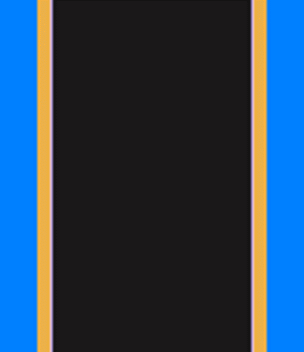
\includegraphics[width=\textwidth]{figs/sec_1a.png}
        \caption{Actual geometry}
        \label{fig_1a}
    \end{subfigure}
    \hspace{6em}
    \begin{subfigure}[b]{0.25\textwidth}
        \centering
        
\includegraphics[width=\textwidth]{figs/sec_1b.png}
        \caption{Discretized geometry}
        \label{fig_1b}
    \end{subfigure}
    \caption{Axial view of a typical Monte Carlo geometry model.}
       \label{fig_1}
\end{figure}

Few methods have been developed to address this issue. One of such method is Localized Delta Tracking (LTD) \cite{nchoi_2020}, which solves radial heat conduction within the fuel pellet using polynomial fitting. This approach allows for the determination of continuously varying radial fuel temperatures. By using LTD within the fuel pellet, MC multi-physics coupling can be achieved without requiring explicit radial discretization of the fuel pellet. However, LTD is limited to handling continuously varying fuel temperatures only in the radial direction. In the axial direction, traditional discretization of the problem domain is still necessary.

Another study by Leppänen \cite{leppanen_2013} modeled nonuniform density distributions using the Serpent 2 MC Code. In this study, he performed MC multi-physics coupling with continuous moderator density combined with the rejection sampling methodology within a single material region. The application considered in this study is related to the continuously varying distribution of coolant density or void fraction along the flow channel of a nuclear fuel assembly. However, this work did not account for variations in temperature and isotopic composition of the material diluted in the moderator, such as boron.

One notable effort was made by Ellis \cite{ellis}, who employed the Functional Expansion Tally (FET) method \cite{chadsey,gries} to achieve continuous representations of power. After multi-physics feedback calculations, the resulting continuous fuel pellet temperature and coolant density were also modeled using functional expansions. To facilitate MC particle tracking in a continuous medium, a modified version of Continuously Varying Material Tracking (CVMT) \cite{brown} was developed. These two methods were integrated to perform MC multi-physics simulations with continuously varying materials.

While Ellis' work and the work presented in this thesis may appear similar, they exhibit several key differences. Firstly, this work successfully develops a technique for calculating the majorant cross-section in a continuous medium, which facilitates delta-tracking and serves as an alternative to CVMT. The use of CVMT introduces complexity by necessitating neutron path integration during particle tracking, thus increasing computational loads. Secondly, this work uses spatial interpolation using a nearly continuous mesh to represent continuous material properties, as opposed to employing FET. This approach reduces the computational burden as it involves fewer arithmetic operations than calculating a complete set of polynomials required by FET. Additionally, the use of spatial interpolation allows that the polynomials are only calculated during physical collisions in delta-tracking method for tallying FET coefficients. Thirdly,  this work introduces an efficient method \cite{honarvar} to calculate Zernike polynomials recursively that marks the first implementation in FET. These distinctions, among others, are summarized in Table \ref{tab_1q}.

\begin{table}
    \centering
    \setlength{\leftmargini}{0.2cm}
    \caption{Key differences between this work and Ellis' work}
    \label{tab_1q} 
    \begin{tabular}{| m{2.75cm} | m{2.75cm} | m{2.75cm} | m{6cm} | }
        \hline
        \multicolumn{1}{|c|}{Aspects} & \multicolumn{1}{c|}{This work} & \multicolumn{1}{c|}{Ellis' work} & \multicolumn{1}{c|}{Remarks} \\
        \hhline{|=|=|=|=|}
        Particle-tracking method & Delta-tracking & CVMT & 
        \begin{itemize} 
            \item Delta-tracking was not used in the Ellis' work because the difficulty in determining majorant XS.
            \item CVMT adds the complexity of neutron path integration during particle tracking.
        \end{itemize} \\
        \hline
        Material properties (i.e., temperature and density) representation & Spatial interpolation using nearly continuous mesh & FET & 
        \begin{itemize} 
            \item Spatial interpolation involves fewer arithmetic operations.
            \item Polynomials are only calculated when the collisions are physical.
        \end{itemize} \\
        \hline
        Zernike polynomials calculations & Uses recursive formula & Uses conventional formula & Marks the first implementation in FET. \\ \hline
        Discretization & Material-wise & Needs discretization when there is spacer grid & This work does not explicit explicit discretization when there is spacer grid. \\ \hline
        Scalability & Whole-core level & Assembly level &  \\ \hline
        Speedup (pin-cell problem) & 4.5 times faster & 1.7 times faster &  \\ \hline
    \end{tabular}
\end{table}

\subsection{Thermal Expansion} \label{sec12}

Thermal expansion (TE) significantly impacts reactor physics modeling, not only for fast reactors but also, to some extent, for LWRs. That is because the reactor design information is typically provided at room temperature, while the actual reactor core operates at much higher temperatures. For instance, at full power, the nominal fuel temperature is around 900 K, and the coolant temperature is approximately 580 K. This substantial temperature difference causes thermal expansion of all components within the reactor vessel. For example, the core plate expands radially, which increases the assembly pitch. The grid spacers within an assembly also expand, altering the pin pitch within the lattice. Additionally, both the fuel pellet and the fuel rod cladding expand in radial and axial directions \cite{palmtag}.

Thermal expansion modeling has long been incorporated into the industry's best-practice two-step methodology for LWR analysis. The two-step methodology involves lattice physics calculations at the assembly level at which the material is homogenized as illustrated in Figure \ref{fig_1x}. In this approach, thermal expansion is accounted for during lattice physics calculations to generate the multi-group cross sections for specific operating reactor temperatures. However, direct MC coupled multi-physics simulations present a challenge: local temperature variations are determined from thermal-hydraulic feedback, and they are not known a priori. Additionally, these temperatures are typically non-uniform within the reactor core.

\begin{figure}
    \centering
    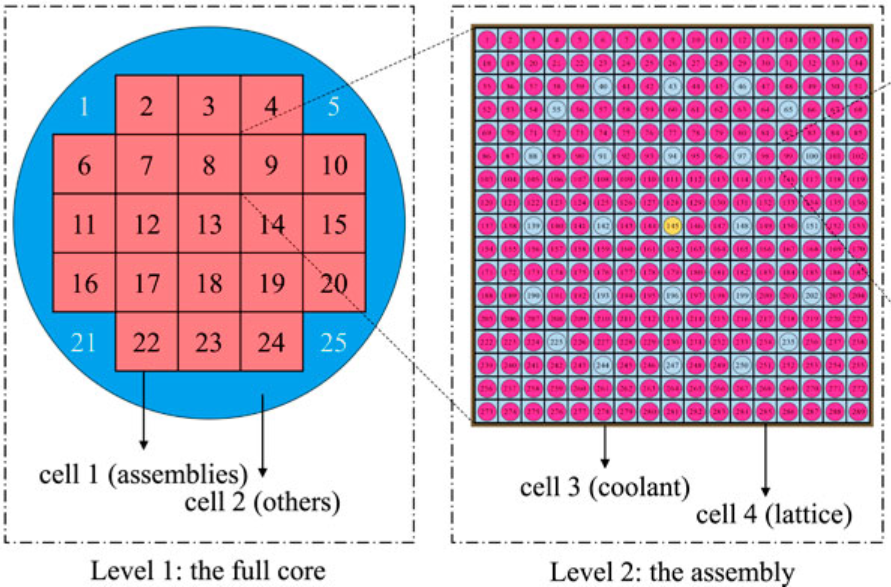
\includegraphics[width=0.65\textwidth]{figs/two_step.png}
    \caption[The two-step methodology for reactor calculations.]{The two-step methodology for reactor calculations. Adapted from \cite{li_2023}}
    \label{fig_1x}
\end{figure}

To address this challenge, typical TE modeling in direct coupled multi-physics simulations is often achieved by manually adjusting input files to uniformly expand the reactor core geometry and modify material densities. This method typically uses core-averaged nominal temperatures, as demonstrated by Palmtag et al. \cite{palmtag}. In Palmtag's work, thermal expansion was implemented by processing XML input files for the Consortium for Advanced Simulation of LWRs (CASL) core simulator code, VERA-CS, to uniformly adjust core dimensions and material densities. This process is accomplished by VERAIn ASCII input preprocessor. However, the VERAIn ASCII input preprocessor only allows thermal expansion at a pre-set, uniform temperature, typically the core-averaged temperature.

Other studies \cite{fiorina,ma_2021,guo} have implemented thermal expansion using thermo-mechanical solvers in Computational Fluid Dynamics (CFD) codes such as OpenFOAM or ANSYS. Generally, these works employed a neutronic solver to obtain power, followed by a CFD code as the TH solver and a mechanical solver to perform material deformation due to temperature changes. However, due to their reliance on direct CFD simulations, these approaches are likely suitable only for small cores, like those in heat pipe or modular reactors. The computational requirements for this method would be exponentially more expensive for larger cores.

Another noteworthy study on reactor simulations with thermal expansion modeling is the work conducted by Idaho National Laboratory \cite{cole_2021}. In this study, they modeled feedback mechanisms that include Doppler effects, radial expansion due to the displacement of the support plate, and axial expansion from the displacement of fuel pins for Unprotected Loss of Flow (ULOF) transient simulations in typical sodium fast reactors. A 2D BISON thermomechanical model of the 316 stainless steel support plate was used to simulate mesh displacement and its effect on the core assembly pitch. Meanwhile, fuel expansion was modeled using a 3D BISON thermomechanical model of the fuel pins. To integrate these models into a multi-physics simulation, they employed the MOOSE multi-app system \cite{moose_2020}, with Griffin, the neutronics solver, serving as the main application.

\subsection{Scope and Objectives}

The objective of this study is to present a framework that enhances the fidelity of typical MC coupled multi-physics simulations for LWRs, through two key improvements. First, the introduction of multi-physics simulations with spatially continuous material properties \cite{imron_2024} to address the spatial resolution issue discussed earlier. Second, the incorporation of on-the-fly thermal expansion of reactor core components during MC particle tracking \cite{imron_otf}.

MC coupled multi-physics simulations with spatially continuous material properties are achieved using FET in combination with delta-tracking. By using delta-tracking instead of CVMT, the complexity of neutron path integration during particle tracking is eliminated. The proposed method is non-intrusive to the thermal-hydraulic (TH) solver, meaning no modifications are required to the TH solver module. This work also adopts an efficient approach from \cite{honarvar} for constructing Zernike polynomials, marking the first use of this method in the application of FET for reactor core simulations.

While the incorporation of thermal expansion is achieved through on-the-fly thermal expansion in MC coupled multi-physics reactor simulations. This method dynamically expands the reactor geometry during particle tracking, enhancing accuracy by using local temperatures, such as pin-averaged or assembly-averaged temperatures, rather than core averaged temperatures. Additionally, as will be shown later in the numerical results section, this approach introduces negligible computational overhead.

This study is limited to static MC coupled multi-physics problems for LWRs. Although the proposed multi-physics framework is applicable to general LWRs, this study specifically focuses on Westinghouse-type Pressurized Water Reactors (PWRs). Additionally, it is restricted to fresh core reactor problems and does not consider depletion or multi-cycle reactor problems. Although spatially continuous depletion is a topic worth exploring, this will be left for future work.

The proposed multi-physics framework in this study has been implemented in the MCS code \cite{hlee_2020} to evaluate its applicability and effectiveness across a range of reactor core problems, from two-dimensional pin-cell models to realistic whole-core reactor problems. MCS is a neutron/photon transport code developed at the Ulsan National Institute of Science and Technology (UNIST), with capabilities for multi-physics and multi-cycle reactor analysis \cite{hlee_2017, yu_2019, yu_2020}.

\subsection{Thesis Outline}

This thesis is structured into five sections. Section \ref{s1} provides the background and motivations for the study. Sections \ref{s2} and \ref{s3} discuss the theoretical framework for MC coupled multi-physics simulations with spatially continuous materials and on-the-fly thermal expansion, respectively. The numerical results are presented and discussed in Section \ref{s4}, which is divided into four major subsections: subsection \ref{sec40} describes the benchmark problem used to evaluate the proposed framework; subsection \ref{sec41} discusses the solutions from multi-physics simulations with spatially continuous material properties; subsection \ref{sec42} focuses on solutions from on-the-fly thermal expansion; and subsection \ref{sec43} presents solutions combining both methodologies. Finally, Section \ref{s5} concludes this thesis and outlines potential future research directions based on the findings.


%%%%%%%%%%%%%%%%%%%%%%%%%%%%%%%%%%%%%%%%%%%%%
%			section 2
%%%%%%%%%%%%%%%%%%%%%%%%%%%%%%%%%%%%%%%%%%%%%
\newpage 
\section{Spatially Continuous Material Properties} 

My second section starts with my equation, which can be written as 
%
\begin{equation}\label{eq:myeq}
\begin{split}
	A 		&= B + C, \\
    D + E	&= F.
\end{split}
\end{equation}
Thus we have (\ref{eq:myeq}).

Fig.~\ref{fig:myfigure} is a sample figure. 

\begin{figure}[h]
\centering
\includegraphics[width=5in]{myfigure.pdf}
\caption{My figure.} \label{fig:myfigure}
\end{figure}

%%%% use the following in the case of eps figure
%\begin{figure} 
%    \centering
%    \epsfig{file=model.eps, width = 0.9\linewidth}
%    \caption{System model with complete bipartite graph. The maximum weighted matching is marked by circles.}
%    \label{fig:model}
%\end{figure}

\subsection{Functional Expansion Tally}
\subsection{Polynomials Calculation}
\subsection{Delta-tracking}
\subsection{Majorant Cross Section Computation}
\subsection{Calculation Flow}


%%%%%%%%%%%%%%%%%%%%%%%%%%%%%%%%%%%%%%%%%%%%%
%			section 3
%%%%%%%%%%%%%%%%%%%%%%%%%%%%%%%%%%%%%%%%%%%%%
\newpage 
\section{Thermal Expansion} 
My third section starts. 

\begin{algorithm}
	\caption{My Algorithm.} \label{algo:myalgo}
    At the beginning ...
    
	\begin{algorithmic}[1]	    
	    \STATE Do this
        \STATE and do this\\
        /* add explanation if necessary */
        \STATE Finally do this
	\end{algorithmic} 
\end{algorithm}
%
Algorithm~\ref{algo:myalgo} is our proposed algorithm.

\begin{table}[!b]
  \centering
  \caption{Solutions for the criticality calculations}
  \label{tab1} 
\begin{adjustbox}{width=1.0\textwidth} % Adjust your table to the text width
  \begin{tabular}{| p{0.05\linewidth} | p{0.1\linewidth} | p{0.1\linewidth} | p{0.1\linewidth} | c | c | p{0.1\linewidth} |}
  \hline 
         &             &                 &                     & \multicolumn{2}{c|}{$k_{eff}$}             &            \\
   \cline{5-6}
   Cases & Boron (ppm) & Bank D Position (steps) & Fully inserted bank & MCS                   & KENO                  & Difference (pcm) \\
   \hline
   1     & 1285        & 167             & -                   & 0.99954 $\pm$ 0.00002 & 0.99990 $\pm$ 0.00001 & -36 $\pm$ 2   \\ \hline
   2     & 1291        & 230             & -                   & 0.99998 $\pm$ 0.00003 & 1.00032 $\pm$ 0.00001 & -34 $\pm$ 3   \\ \hline
   3     & 1270        & 97              & Bank A              & 0.99836 $\pm$ 0.00003 & 0.99880 $\pm$ 0.00001 & -44 $\pm$ 3   \\ \hline
   4     & 1270        & 113             & Bank B              & 0.99900 $\pm$ 0.00003 & 0.99936 $\pm$ 0.00001 & -36 $\pm$ 3   \\ \hline
   5     & 1270        & 119             & Bank C              & 0.99863 $\pm$ 0.00003 & 0.99904 $\pm$ 0.00001 & -41 $\pm$ 3   \\ \hline
   6     & 1270        & 18              & Bank D              & 0.99871 $\pm$ 0.00003 & 0.99908 $\pm$ 0.00001 & -37 $\pm$ 3   \\ \hline
   7     & 1270        & 69              & Bank SA             & 0.99857 $\pm$ 0.00003 & 0.99902 $\pm$ 0.00001 & -45 $\pm$ 3   \\ \hline
   8     & 1270        & 134             & Bank SB             & 0.99897 $\pm$ 0.00004 & 0.99932 $\pm$ 0.00001 & -35 $\pm$ 4   \\ \hline
   9     & 1270        & 71              & Bank SC             & 0.99910 $\pm$ 0.00003 & 0.99898 $\pm$ 0.00001 & 12  $\pm$ 3   \\ \hline
   10    & 1270        & 71              & Bank SD             & 0.99916 $\pm$ 0.00003 & 0.99898 $\pm$ 0.00001 & 18  $\pm$ 3   \\ \hline
  \end{tabular}
  \end{adjustbox}
\end{table}

\subsection{Theory}
\subsection{Thermal Expansion Coefficients}
\subsection{On-the-fly Thermal Expansion}
\subsection{Calculation Flow}


%%%%%%%%%%%%%%%%%%%%%%%%%%%%%%%%%%%%%%%%%%%%%
%			section 4
%%%%%%%%%%%%%%%%%%%%%%%%%%%%%%%%%%%%%%%%%%%%%
\newpage 
\section{Numerical Results} 
\subsection{Spatially Continuous Material Properties}
\subsubsection{Two-dimensional Pin-cell Problem}
\subsubsection{Three-dimensional Pin-cell Problem}
\subsubsection{Three-dimensional Assembly Problem}
\subsubsection{Whole-core Reactor Problem}

\subsection{Thermal Expansion}
\subsubsection{Assembly Problem}
\subsubsection{Whole-core Reactor Problem}
\subsubsection{Isothermal Temperature Coefficient}
%\subsubsection{Whole-core Reactor Depletion using Restart Calculations}

\subsection{Combined Framework}
\subsubsection{Assembly Problem}
\subsubsection{Whole-core Reactor Problem}
%\subsubsection{Whole-core Reactor Depletion using Restart Calculations}


%%%%%%%%%%%%%%%%%%%%%%%%%%%%%%%%%%%%%%%%%%%%%
%			Conclusion
%%%%%%%%%%%%%%%%%%%%%%%%%%%%%%%%%%%%%%%%%%%%%
\newpage 
\section{Conclusion} 
My conclusion here.

\clearpage

%%%%%%%%%%%%%%%%%%%%%%%%%%%%%%%%%%%%%%%%%%%%%
%			Reference
%%%%%%%%%%%%%%%%%%%%%%%%%%%%%%%%%%%%%%%%%%%%%
\addcontentsline{toc}{section}{References}
\bibliographystyle{IEEEtran}
\bibliography{main.bib}
\clearpage

%%%%%%%%%%%%%%%%%%%%%%%%%%%%%%%%%%%%%%%%%%%%%
%			Acknowledgements
%%%%%%%%%%%%%%%%%%%%%%%%%%%%%%%%%%%%%%%%%%%%%
\addcontentsline{toc}{section}{Acknowledgements}
\section*{\hfill \Large Acknowledgements \hfill}
First and foremost, I am deeply grateful to Allah for His endless mercy and blessings throughout this journey. His grace has given me strength through all the challenges.

I would like to express my sincere thanks to my advisor, Prof. Deokjung Lee, for his invaluable advice, continuous encouragement, and financial support during my study in the CORE Laboratory. I am deeply grateful for the opportunity he provided me to study in his laboratory. Studying and working in the CORE Laboratory has opened new horizons of knowledge for me.

I also want to extend my appreciation to the members of my dissertation committee. Their thoughtful feedback and constructive criticism have greatly helped in refining my work and pushing me to achieve better results. My gratitude also extends to the staff at the Department of Nuclear Engineering at Ulsan National Institute of Science and Technology (UNIST).

I am also grateful to my lab mates for their friendship, insightful discussions, and moral support. Their companionship has been a source of strength during tough times and has made the long hours in the lab much more enjoyable. 

To my beloved parents, I cannot thank you enough. Your unconditional love, support, and prayers have been my constant source of motivation. Your sacrifices and unwavering belief in me are beyond words, and I dedicate this achievement to you.

Finally, I want to thank my family, especially my dear wife. Her love, patience, and strength have been my greatest support throughout this journey. She took care of our four sons while living abroad with me during my studies, and her dedication and sacrifice have made this accomplishment possible.

I would also like to express my thanks to everyone who has supported me in any way during this journey. Your help and encouragement have meant the world to me.
\clearpage

%%%%%%%%%%%%%%%%%%%%%%%%%%%%%%%%%%%%%%%%%%%%%%%%%%%%%%%%%%%%% 
%%%%%%%%%%    Do not touch the below 
%%%%%%%%%%%%%%%%%%%%%%%%%%%%%%%%%%%%%%%%%%%%%%%%%%%%%%%%%%%%% 

%%% The following page is intentionally left as blank
% White attachment form
\hbox{ }
\thispagestyle{empty}
\clearpage

\end{document}

